We corrupt the depth channel at test time for both depth policies (3 amplitudes, 20 held-out terrains each; Table~\ref{tab:h2}, Fig.~\ref{fig:h2}). Corruptions: Gaussian noise ($\sigma_n=0.05,0.15,0.30$ in normalised depth, i.e.\ up to 30\,cm), 20\% pixel dropout, a square occluder covering 25\% or 50\% of each image, and a ``blank'' control where every pixel is invalid.

\begin{table*}[t]
\centering\caption{H2: depth corruption at test time (all amplitudes pooled).}\label{tab:h2}
\small\begin{tabular}{llcccc}\toprule
Policy & Condition & $n$ & Success [\%] & Fall [\%] & Return\\\midrule
Prop.+depth & blank & 120 & 70 & 28 & 131.3 \\
Prop.+depth & clean & 120 & 69 & 28 & 131.3 \\
Prop.+depth & dropout 0.2 & 120 & 70 & 28 & 131.3 \\
Prop.+depth & noise 0.05 & 120 & 69 & 28 & 131.3 \\
Prop.+depth & noise 0.15 & 120 & 69 & 28 & 131.3 \\
Prop.+depth & noise 0.30 & 120 & 70 & 28 & 131.3 \\
Prop.+depth & occlusion 0.25 & 120 & 69 & 28 & 131.3 \\
Prop.+depth & occlusion 0.50 & 120 & 70 & 28 & 131.3 \\
\bottomrule\end{tabular}\end{table*}


\begin{figure}[t]
\centering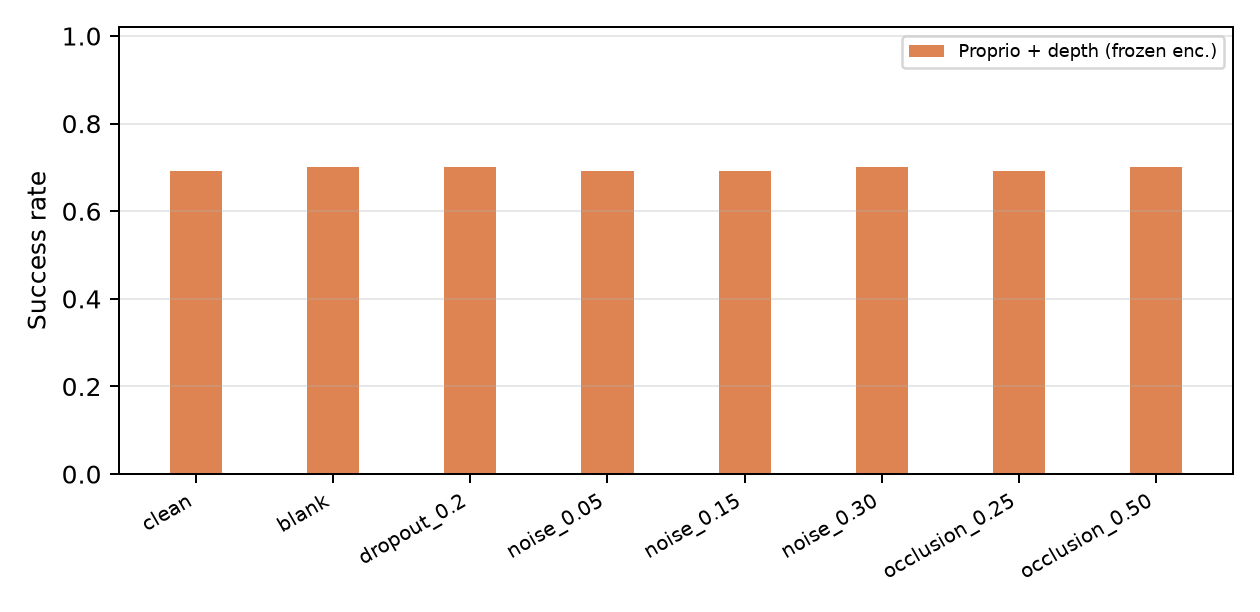
\includegraphics[width=\columnwidth]{figures/h2_robustness.png}
\caption{H2: success under depth corruption (depth policies; dashed line: proprio-only, clean).}\label{fig:h2}
\end{figure}

\textbf{Result.} Success and fall rates are unchanged by every corruption (all paired differences from the clean condition are within $\pm0.01$, $p\ge0.32$; Table~\ref{tab:tests}), \emph{including the blank-depth control}. We verified that the corruption does reach the policy (a $\sigma_n{=}0.3$ perturbation changes the observed image by 0.18 on average; the blank condition sets every pixel to 1). H2's premise, that performance drops when vision is degraded, is therefore \textbf{not observed}, and the reason is informative: the trained policies do not use the depth features. The $+$depth policies behave like proprioception-only policies with extra, ignored inputs, which is consistent with the H1 result. Plausible causes are that the terrains in the training range are shallow enough for proprioceptive feedback to suffice, that the frozen encoder was pretrained on a different terrain distribution, and the short training budget; these are tested in the next steps (Sec.~\ref{sec:concl}).
